\documentclass[letterpaper,abstract=on,titlepage=false]{scrreprt}
%Report without title page, Abstract has a special title
\usepackage[T1]{fontenc}
\usepackage{graphicx}
\usepackage{float}
\usepackage{lmodern} %Better fonts
\graphicspath{ {img/} }

\begin{document}
\title{Programatically Predicting Bus Occupancy}
\subtitle{Undergraduate Independent Research Report}
\author{Daniel Bordak, Erin Corrado, Revan Sopher, and Ashley Weaver}

\maketitle

\begin{abstract}
In this study we address the problem of programatically predicting bus occupancy.
We approach this in two ways: by using publicly available GPS positions to calculate stop time, and by using promiscuous Wi-Fi to count devices.
While the stop time approach proved unfruitful due to the significant time requirement in establishing a benchmark by which to interpret the data, the Wi-Fi approach yielded an accurate model once we compensated for noise.
We conclude by suggesting modifications to the experiment, and the application of this methodology to the determination of occupancy of other locales.
\end{abstract}

\section*{Motivation}

Due to the periodic nature of class schedules, students at Rutgers tend to move between campuses in certain known time intervals during the day.
This leads to predictable migratory patterns; however, the bus schedule does a poor job of taking student schedules into account. 
On Livingston campus, for example, the College Ave/Livingston buses circulate consecutively yet are nearly empty, while the Busch/Livingston buses are less frequent and are often packed to capacity.
The aim of this project is to develop a system for better predicting the demand for buses, such that an empirical argument for the optimization of the bus schedule might be made.

\section*{Approach}

In order to facilitate simultaneous contributions from all four team members, we approached the problem in two manners: by directly collecting data about number of riders vs. stop time, and by measuring number of devices on the bus.
Two students worked on each approach, and we planned to combine results into a single prediction method.

	\subsection*{Stop Length Inference}

	In this approach, we planned to establish a correlation between the length of time a bus spends at a stop and the number of passengers currently riding it, our theory being that as a bus nears capacity, stops will be longer due to the larger number of riders entering and exiting.
	Every Rutgers bus periodically updates an internet source with its position, velocity, and destination.
	This information is publicly available, not requiring any hardware or observers on the bus, therefore lending itself to zero-cost large-scale execution.
	We first tried to measure the strength of this correlation; if we could prove a strong positive correlation, we could use the bus travel data to measure length of stops, and therefore predict occupancy.
	Although this method inherently depends on a weaker correlation than the number of smartphones, by running the analysis on a log of travel data, we could predict occupancy across a significantly larger domain and for no cost.

	\subsection*{Promiscuous WiFi}

	In this approach, we used the inherent correlation between the number of smartphones on the bus and the number of passengers: more devices logically implies more passengers, because the devices travel with the passengers.
	We hold that this correlation is fundamental enough to not require investigation such as in the previous approach.

	We used a laptop running Linux and equipped with a standard wireless card and a GPS sensor.
	The computer ran the wireless card in monitor mode.
	In normal operation, a wireless card will receive every packet in the vicinity, but discard those that are not specifically addressed to it; in monitor mode all received packets are transmitted to the operating system regardless of intended recipient.
	The laptop logged the headers of these packets to a file.
	The log contained time (accurate to the microsecond), source and destination MAC addresses, and signal strength.

\section*{Results}

\subsection*{Stop Length Inference}
	In order to establish a correlation between stop length and bus occupancy, we followed a bus on its circuit, recording data about its stops, namely, the number of people either boarding or exiting the bus and the length of the stop.
	\begin{figure}[H]
	\includegraphics[width=11cm]{stop3}
	\centering
	\end{figure}
	As we quickly found, stop length does not appear to have any correlation to occupancy.
	This makes sense, because the number of sedentary riders does not cause slowdowns; rather, the relevant metric is the number of people entering or exiting the bus.

	\begin{figure}[H]
	\includegraphics[width=11cm]{stop1}
	\centering
	\end{figure}

	Plotting the net occupancy change as a function of stop length was also inconclusive, as the longer stops could signify either positive or negative changes.
	From stop timings alone, we would not be able to predict the direction of change.

	\begin{figure}[H]
	\includegraphics[width=11cm]{stop2}
	\centering
	\end{figure}

	Net change, however, shows a stronger correlation, confirming our hypothesis that high rider throughput causes delays.
	Net change is not a useful metric on its own, but if it could be proven that certain bus stops tended to have a generally positive or negative net change, we could predict the sign of the change and thus the occupancy changes over time.
	% for example, more people tend to get on at the [whatever] than get off, so a longer stop at here means a large positive change
	% conversely, the bus stop at [whatever] tends to have a negative net change, so a longer stop here would mean that there were fewer people on the bus afterwards
	\\
	To test this, we waited at a single bus stop and counted the number of passengers entering and leaving each bus on a certain route, and the length of the stops.

	%TODO:
	\begin{figure}[H]
	GRAPH OF CHANGE AT SINGLE STOP GOES HERE
	\centering
	\end{figure}
	% either add a title to this graph or remove the title from all the other graphs

	Data for this experiment was slower to collect, as the buses were spaced out.
	This data suggests that this bus stop is predominantly a descent spot; thus, longer stops at this stop would imply a net decrease in number of riders.
	\\
	However, the data collected is insufficient to draw these conclusions; there can be significant variation depending on time and day of the week.
	This data collection would need to be repeated at every bus stop, on a variety of days and times, in order to provide the required basis of prediction.
	This clearly increases the time requirement to well beyond the scope of this study.
	\\
	Thus, while the preliminary foray suggests that this approach is tentatively successful, it is not feasible for this study.
	We move on to our next approach.


\subsection*{Promiscuous WiFi}
	To collect data, we put a laptop's wireless card into monitor mode and ran the following command:
	\begin{verbatim}
		tcpdump -e
	\end{verbatim}
	This command logs the headers of every packet that the wireless card sees, thus uniquely identifying every active device in the area.
	We followed a bus on its route, logging packets and stop times.
	tcpdump also records the strength of signals, so we can choose to ignore packets below a certain decibel strength.

	\subsubsection*{Packet Plot}

		\begin{figure}[H]
		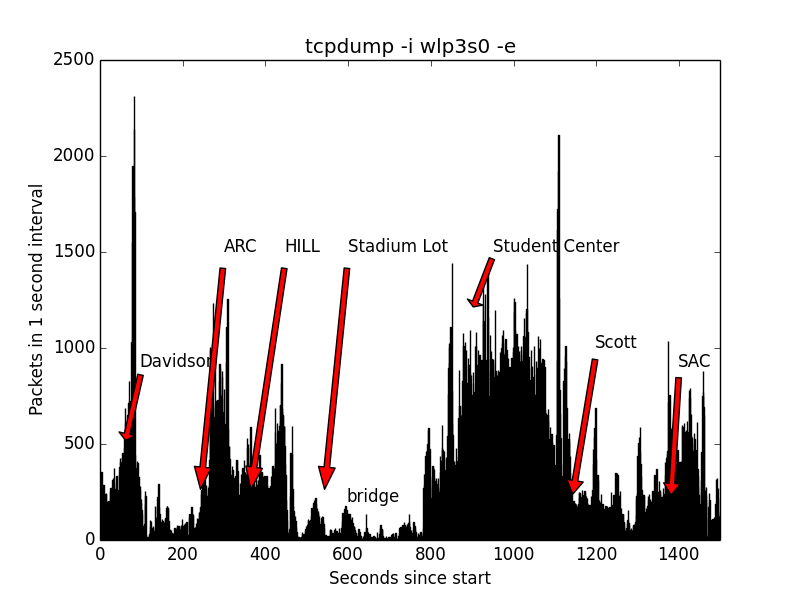
\includegraphics[width=11cm]{packets}
		\\TODO: swap out plot for new data
		\centering
		\end{figure}

		Plotting the number of packets in a histogram with one second bins, we see that there are visible differences between stops.
		There are a few extreme spikes in network traffic, which can be ignored as extraneous points.
	
	\subsubsection*{Unique MAC Plot}

		Network traffic is not a good indicator of occupancy, however, because it is highly susceptible to the noise of a single user transmitting many packets.
		Instead, we switched out ``number of packets'' for ``number of unique MAC addresses''.
		As an additional filter we can eliminate all MAC addresses that are access points, because access points periodically broadcast their existence and will thus cause noise.

		\begin{figure}[H]
		\includegraphics[width=16cm]{bus-unique-no-filtering}
		\\TODO: remake with strength cutoff, step function overlay, fix spelling of Scott
		\centering
		\end{figure}

		The values on this plot differ noticeably between stops.
		However, this is not due to occupancy; there are clearly not nearly that many people on the bus.
		Instead, it seems that the shape of the plot is primarily influenced by the geographic area: the portions of the bus loop by athletic fields and between campuses has nearly no data.

	\subsubsection*{First-Last Grid Plot}
		In order to establish which devices were on the bus, we plotted the time of the first and last occurrence of each device:

		\begin{figure}[H]
		\includegraphics[width=16cm]{bus-grid-no-filtering}
		\\TODO: remake with strength cutoff, fix spelling of Scott
		\centering
		\end{figure}

		Each point here represents a unique device, where the x-coordinate is the time of the first sighting, and the y-coordinate is the time of the last sighting.
		Thus, the high concentration of data points along the line y=x represents the transient devices, most likely people outside.
		The clump of data points in the top left corner of the plot represents devices which were seen throughout the journey. 
		These are most likely our own devices, or stationary devices around the common first and last stop.

	\subsubsection*{Presence Vector Plot}
		In an attempt to minimize noise from the above transient devices and to compensate for the lack of traffic in uninhabited areas, we construct a plot similar to the previous.
		For every address we encountered in the collection, we create a vector defined by the following function:
		\begin{displaymath}
		f(x) = \left\{
			\begin{array}{lr}
			1 & if firstSighting \le x \le lastSighting\\
			0 & otherwise
			\end{array}
		\right.
		\end{displaymath}

		We sum these vectors into a single vector, where the value at any point indicates how many devices we can infer are presently on the bus.

		\begin{figure}[H]
		\includegraphics[width=17cm]{bus-vectors-wide}
		\centering
		\end{figure}

		Overlaid on this plot is the step function corresponding to the observed number of riders.
		It is scaled differently, as there is approximately a three time difference between the devices seen and the people riding.
		\\
		We see that there appears to be an excellent correlation here, with the exception of the 400-700 second segment.
		This segment corresponds to the entrance to the College Avenue campus, a highly concentrated area which appears to have contributed considerable noise.
		We do see, however, that the two changes in occupancy in this region seem to correspond to peaks in the traffic -- this means that the traffic is probably a flat-rate higher in that area, which we can account for in prediction.
		\\\\
		Thus, we can conclude that this approach is successful.

%\section*{Conclusion}
%	From the data above, we determined that the occupancy of a bus could be predicted by observing data traffic with some sensor placed on the bus.
%	We can filter out some of the irrelevant data by ignoring any signals below a certain strength.
%	This is the most feasible method, but requires external assistance with installation of devices.


\section*{Future Work}
\subsection*{Continuation of Benchmark}
	The Stop Length Inference approach seemed promising, but we would need to benchmark every stop several times in order to be able to know which direction of occupancy change a long stop indicates. Thus, there is substantial opportunity to complete this benchmarking in order to complete that approach.
\subsection*{Change of Approach}
	The largest problem with the interception of packets is outside noise.
	To address this, we would like to install an access point on the bus, with the same SSID as the campus Wi-Fi so that smart phones would automatically connect.
	We could then listen only to communications with this access point, eliminating outside traffic.
	\\
	Optimally, the routers would be officially installed and serve mobile data. 
	This is naturally expensive and thus unlikely. 
	Any unofficial access points installed would be an explicit violation of the terms of use of the Rutgers networks, and thus unfeasible as well.
	\\\\
	We could also replace the laptop in our setup with a smaller unit to be installed in the buses, to collect data for longer periods of time. 
	Running several of these units would allow us to collect enough data to make occupancy predictions.

\subsection*{Change of Application}
	While we initially set out to programatically predict the occupancy of buses, the Promiscuous Wi-Fi approach is also applicable to the determination of the occupancy of other scenarios.
	To demonstrate, we ran tcpdump for twenty minutes during a lecture, and followed a similar analysis procedure.
	The concept of "stops" doesn't apply to this situation, however we can still derive interesting results.

	\begin{figure}[H]
		\includegraphics[width=12cm]{prob-grid-final}
		\centering
		\\TODO: Title "Lecture"
	\end{figure}

	As before, the points around y=x consist of transient devices.
	The points in the clump to the top right is probably due to a buildup of students outside the lecture hall awaiting the following class.
	The points in the clump to the top left represent the devices that were present for the duration of the capture.
	\\
	There were exactly 106 students in the lecture hall during this collection; while determining the exact boundaries is of a complexity outside the scope of this project, the clump in the top left contains approximately 100 points.
	This suggests that this approach does generate an accurate count of the lecture hall occupancy.

	\begin{figure}[H]
		\includegraphics[width=17cm]{packethist-log}
		\centering
		\\TODO: Replace with sorted version
	\end{figure}

	In this plot we see that we can partition devices into classes based on how frequent the packets.
	While a small number of devices were generating enormous amounts of network traffic with millions of packets, others generated orders of magnitude fewer.
	\\\\
	This suggests another interesting path of inquiry: monitoring the interest of an audience based on network traffic.
	The assumption here is that a bored audience is more likely to cause network traffic by web browsing.

\chapter*{Team Member Contributions}
Daniel Bordak
\begin{itemize}
  \item Collected tcpdump and classroom data
  \item Created tcpdump output parser used in all plots (not yet in report)
  \item Optimized graph plotting functions for speed
  \item Cowrote First-Last Grid Plot
  \item Cowrote Segments Plot (not in report)
  \item Rewrote Unique Device Plot and Packet Plot to allow for different binsizes (not yet in report)
  \item Wrote Stop-Time parser for use in plot annotations.
\end{itemize}
Erin Corrado
\begin{itemize}
  \item Collected bus and classroom data
  \item Cowrote First-Last Grid Plot
  \item Wrote length/occupancy correlation plot
  \item Cowrote poster
\end{itemize}
Revan Sopher
\begin{itemize}
  \item Wrote Proposal
  \item Collected tcpdump data
  \item Wrote Raw Packet Plot
  \item Wrote Unique Device Plot
  \item Cowrote Segments Plot (not in report)
  \item Wrote Vector Plot
  \item Wrote Report
\end{itemize}
Ashley Weaver
\begin{itemize}
  \item Collected bus data
  \item Cowrote Poster
  \item Commented on report
\end{itemize}
\end{document}
